\section{Resultados e discussão}

Para encontrar todos os resultados necessários para comprovar a teoria, a prática foi dividida em algumas etapas, sendo elas:


\begin{itemize}

    \item Montar o circuito da figura \ref{ckt:1} e variar $V_{in}$ na entrada e verificar com multímetro a tensão de saturação positiva e negativa, obtida na saída do circuito. 
    
    \item Variar a entrada de modo a encontrar a tensão de offset do CI LM741;
    
    \item Repetir o primeiro passo no circuito da figura \ref{ckt:2}.
    
    \item Aplicar um $V_{in} = 2sen (2\pi\times150\times t)$ obter a curva de histerese (CT do circuito), com as tensões limiares do circuito.
\end{itemize}

Primeiramente foi montado o circuito comparador não-inversor simples, desse modo foram obtidos suas tensões de saturação na saída variando a tensão $V_{in}$ na entrada de modo a obter na saída $V_{sat}^+$ e $V_{sat}^-$, a utilização dos diodos emissores de luz (LEDs), foi feita apenas para melhor entendimento e visualização do experimento. 

\begin{center}
        $V_{sat}^+ = +8.586$ V
\end{center}
\begin{center}
        $V_{sat}^- = -8.586$ V
\end{center}

Observa-se que devido as perdas internas do próprio AMPOP (LM741), obtemos uma saída diferente da ideal que é $\pm 10V$.

A medição da tensão do \textit{input offset} do CI LM741 é para temperatura padrão (25ºC) em torno 5mV, a medição desse valor foi realizada variando a entrada de modo a se estabilizar em torno do ponto de transição das duas margens de saturação. Foi obtido o valor de aproximadamente:

\begin{center}
        $V_{of} = 3.43$ mV
\end{center}

Assim, a característica de transferência prática pode ser observada na figura \ref{graph:3} com o \textit{offset} na tensão de referência.


\begin{figure}[H]
\begin{center}
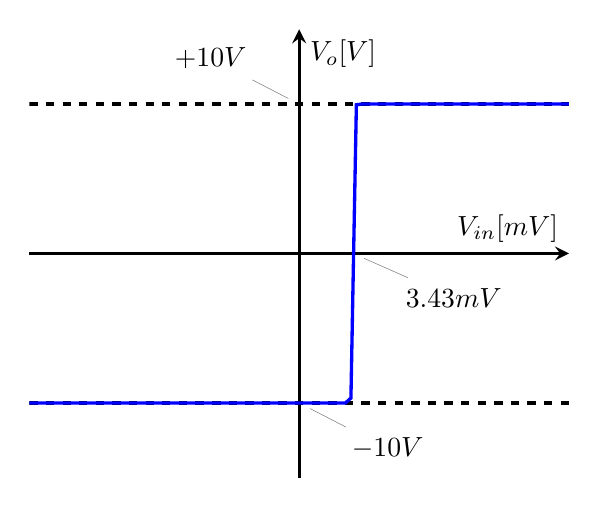
\begin{tikzpicture} 
\begin{axis}[very thick,
                     samples = 100,
                     ytick={-10,10},
                     xlabel = {$V_{in}[mV]$},
                     ylabel = {$V_{o}[V]$},
                     xmin = -5,
                     xmax = 5,
                     ymin = -15,
                     ymax = 15,
                     axis x line = middle,
                     axis y line = middle,
                     ticks = none]
            \addplot[dashed] plot (\x, 10);
            \addplot[dashed] plot (\x,-10);
            \addplot[blue] plot (\x, {-10+20/(1 + exp(-(\x-1)*100))});
            \addplot[mark=none] coordinates {(0,10)} node[pin=150:{$+10V$}]{};
            \addplot[mark=none] coordinates {(0,-10)} node[pin=-30:{$-10V$}]{};
            \addplot[mark=none] coordinates {(1,0)} node[pin=-30:{$3.43mV$}]{};
        \end{axis}
\end{tikzpicture}
\end{center}
\caption{Característica de transferência para o comparador não inversor simples.}
\label{graph:3} 
\end{figure}

Esse valor é aceitável pois no \textit{datasheet} do LM741 é previsto uma \textit{input offset voltage} de no máximo 5mV.

Foi utilizado em ambos os circuito o potenciômetro em série com dois resistores de $10k\ohm$, de modo a diminuir a faixa das tensões de entrada de  $\pm 10V$ para em torno de  $\pm 3.3333V$, de modo que o ajuste seja mais fácil e preciso.

Na segunda parte do experimento foi montado o circuito comparador regenerativo "Schmitt Trigger", que nada mais é que um comparador inversor com histerese, e que deve ser medido as tensões de saturação do circuito na saída, que por se tratar do mesmo CI e da mesma tensão $V_{in}$ e referência de entrada (Terra) ter-se-á praticamente os mesmo valores encontrados na circuito da figura \ref{ckt:1}. Logo:

\begin{center}
        $V_{sat}^+ = +8.73$ V
\end{center}
\begin{center}
        $V_{sat}^- = -8.555$ V
\end{center}

Em seguida, para medição das tensões de limiar, foi necessário retirar o potenciômetro e no local colocar um onda senoidal $2V_{pico}$ e frequência de 150Hz. Com isso possível obter a onda resultante na saída, que é uma onda quadrada nos valores de $V_{sat}^+$ e $V_{sat}^-$ como é mostrada na figura \ref{fig1} abaixo:


\begin{figure}[H] 
\centering
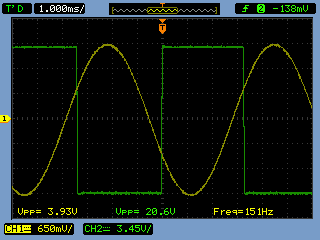
\includegraphics[width=7.5cm]{images/time.png}
\caption{Comparação entre entrada e saída no tempo.}
\label{fig1} 
\end{figure}

Pode-se identificar na figura \ref{fig1} que a onda quadrada resultante está defasada em relação à senoide. Isso é devido a mudança de nível da onda quadrada apenas quando encontra-se com a onda senoidal em que seu valor de tensão obedeça o valor de transição.

Para a análise da CT e obtenção das tensões limiares experimentais, foram utilizados o modo X-Y da osciloscópio de modo a obter a curva da figura \ref{fig2}.

\begin{figure}[H] 
\centering
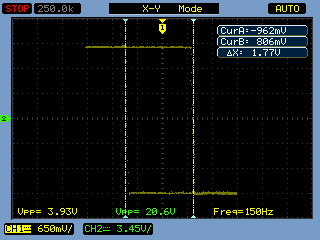
\includegraphics[width=7.5cm]{images/xy_cursors.png}
\caption{Característica de transferência prática.}
\label{fig2} 
\end{figure}

Da figura \ref{fig2} extrai-se que os valores de transição são: $V_1=-962mV$ e $V_2=806mV$. Antes de inserir a onda de tensão senoidal, foi ajustado o potenciômetro para obter as tensões de transição, que foram: $V_1=-1.058V$ e $V_2=966mV$. Percebe-se que, as tensões limiares encontradas na prática são muito próximas ao valores teóricos encontrados e próximas entre si, considerando que os valores encontrados no osciloscópio são mais precisos do que aqueles ajustados manualmente.

Na imagem acima, pode-se notar que quando se aumenta a tensão de entrada, a saída saturará no valor de saturação positivo quando ultrapassar o limiar superior, de forma análoga, ocorrerá a mesma coisa para quando o valor é diminuído na entrada, dessa forma, só saturará quando a entrada estiver abaixo do limiar de comparação inferior. Dessa forma, percebemos que a figura em questão é bastante parecido a CT teórica apresentada. 



